\begin{chapter}{\label{cha:numerics}Numerical Algorithms}
\section{\label{section:RK} Numerical procedures for 2D and 3D solutions}
	\subsection{\label{section:RK4} Fourth order Runge-Kutta scheme}
	The classical fourth-order Runge-Kutta formula (RK4) is described equivalently in many texts. We follow the description in \cite{NumericalRecipes}. Let an initial value problem be specified as
	
	\begin{align*}
		\frac{\partial \psi}{\partial t} &= f(\psi,t),\hspace{0.25in}\psi(t_0) = \psi_0.
	\end{align*}

A step-size, $h>0$, is chosen as the parameter controlling how the solution is advanced over $t$. The scheme for estimating $\psi(t_n)= \psi_n$ is then written
\begin{equation}
\begin{split}
		k_1 &= hf(t_n,\psi_n),\\
		k_2 &= hf(t_n+\frac{h}{2},\psi_n+\frac{k_1}{2}),\\
		k_3 &= hf(t_n+\frac{h}{2},\psi_n+\frac{k_2}{2}),\\
		k_4 &= hf(t_n+h,\psi_n+k_3),\\
		\psi_{n+1} &= \psi_n + \frac{k_1}{6}+ \frac{k_2}{3}+ \frac{k_3}{3} + \frac{k_4}{6} + \mathcal{O}(h^5),\\
		t_{n+1}  &= t_n + h.
		\label{eq:rk4}
\end{split}
\end{equation}


	An outline derivation of the Runge-Kutta scheme, which includes a proof of accuracy are shown in Appendix \ref{appsection:rk4deriv}.
	In all of our relevant calculations the value of f is set as the right hand side of the homogeneous or trapped GPE. The main loop formulating the RK4 method may be repeated indefinitely to reach any $t>t_0$. The step size for a given set of parameters should be chosen small enough that smaller choices make no quantitative changes to the resulting solution. The following section outlines the methods we have implemented to ensure numerical solutions are converged.

	\subsection{\label{section:numericalParams} Numerical stability and convergence}
	We now investigate numerical parameters which affect the stability of simulated superfluid systems. Our direct aim is to find a suitable discretisaton of space and time so that while simulations are timely, our numerical quantities are converged, that is, not overly sensitive to small changes in computational parameters and that quantities conserved by the equations of motion are indeed conserved in the computed numerical solutions.

	We begin by estimating the required distance between our grid points, $\Delta$, in a homogeneous system by considering the width of the vortex core, a feature we would like well and accurately visualised in our numerical solutions. Through observation of a singly quantised vortex core (as in Figure \ref{fig_vortex}) we observe a core radius of approximately $5\xi$ when the background density is $\rho=1$. To ensure the vortex core structure is well resolved we decide to dedicate 10 grid points for a vortex core radius, suggesting a value of $\Delta = \xi/2$.

	\begin{figure}
	\centering
   \begin{tikzpicture}
    \begin{axis}[y tick label style={
		        /pgf/number format/.cd,
		            fixed,
		            fixed zerofill,
		            precision=3,
		        /tikz/.cd
		    },
        width=0.98\linewidth,
        height=0.3\linewidth,
        xlabel={},
        ylabel=$\hat{E}\left ( \hat{t} \right )$,
        xmin=0,
        xmax=10,
        major tick length = 0.07cm
      ]
      \addplot gnuplot [raw gnuplot,mark=none,color=black,thick]{
      	plot "numerics/figures/energ-norm-cons.0.05" using 1:3 with lines;
      };
      \addplot gnuplot [raw gnuplot,mark=none,color=red,thick]{
      	plot "numerics/figures/energ-norm-cons.0.1" using 1:3 with lines;
      };
      \addplot gnuplot [raw gnuplot,mark=none,color=green,thick]{
      	plot "numerics/figures/energ-norm-cons.0.2" using 1:3 with lines;
      };
      \addplot gnuplot [raw gnuplot,mark=none,color=blue,thick]{
      	plot "numerics/figures/energ-norm-cons.0.4" using 1:3 with lines;
      };
    \end{axis}
  \end{tikzpicture}
  \begin{tikzpicture}
    \begin{axis}[y tick label style={
		        /pgf/number format/.cd,
		            fixed,
		            fixed zerofill,
		            precision=4,
		        /tikz/.cd
		    },
        width=0.98\linewidth,
        height=0.35\linewidth,
        name=mainplot,
        xlabel=$\hat{t}$,
        ylabel=$\hat{N}\left ( \hat{t} \right )$,
        xmin=0,
        xmax=10,
        ymax=1.0008,
        major tick length = 0.07cm
      ]
      \addplot gnuplot [raw gnuplot,mark=none,color=black,thick]{
      	plot "numerics/figures/energ-norm-cons.0.05" using 1:4 with lines;
      };
      \addplot gnuplot [raw gnuplot,mark=none,color=red,thick]{
      	plot "numerics/figures/energ-norm-cons.0.1" using 1:4 with lines;
      };
      \addplot gnuplot [raw gnuplot,mark=none,color=green,thick]{
      	plot "numerics/figures/energ-norm-cons.0.2" using 1:4 with lines;
      };
      \addplot gnuplot [raw gnuplot,mark=none,color=blue,thick]{
      	plot "numerics/figures/energ-norm-cons.0.4" using 1:4 with lines;
      };
      \node[anchor=west] (source) at (axis cs:9.7,1.00025){};
      \node[anchor=west] (destination) at (axis cs:9.7,1.0000){};
      \draw[->](source)--(destination);
    \end{axis}
    \begin{axis}[y tick label style={
		        /pgf/number format/.cd,
		            fixed,
		            fixed zerofill,
		            precision=6,
		        /tikz/.cd
		    },
        width=0.4\linewidth,
        height=0.18\linewidth,
        at={(mainplot.north east)},anchor=north east,
        xlabel={},
        ylabel={},
        xmin=9,
        xmax=9.999,
        major tick length = 0.07cm
      ]
      \addplot gnuplot [raw gnuplot,mark=none,color=black,thick]{
      	plot "numerics/figures/energ-norm-cons.0.05" using 1:4 with lines;
      };
      \addplot gnuplot [raw gnuplot,mark=none,color=red,thick]{
      	plot "numerics/figures/energ-norm-cons.0.1" using 1:4 with lines;
      };
      \addplot gnuplot [raw gnuplot,mark=none,color=green,thick]{
      	plot "numerics/figures/energ-norm-cons.0.2" using 1:4 with lines;
      };
    \end{axis}
  \end{tikzpicture}
  \caption{Dimensionless energy, $\hat{E}$, and particle number, $\hat{N}$, throughout numerical propagation of a trapped condensate containing a singly quantised vortex in its center, with interaction energy $\hat{g}=2000$ and chemical potential $\hat{\mu}=25.27$. The numerical grid width varies with each line; (black) $\Delta = 0.05$, (red) $\Delta = 0.1$, (green) $\Delta = 0.2$ and (blue) $\Delta = 0.4$. (Inset) Zoomed view of the convergence of $\hat{N}$.}\label{fig_energ_norm_cons}
 \end{figure}

	In the trapped case we can use the same idea. It is shown in Section \ref{section:healing} that $\xi = \hbar/\sqrt{mg}$ for $\rho=1$. We can then easily rearrange to find an expression for $\xi$ in the harmonic oscillator units of trapped condensates. We find that our approximate grid spacing to adequately resolve the vortex core is $\Delta = 0.5\xi = 0.5\omega \sqrt{\hbar/(\mu \omega)} l_r$. As an example, for a trapped condensate with interaction energy $\hat{g}=2000$, chemical potential $\hat{\mu}=25.27$ and trap frequency $\omega=8.75~{\rm Hz}$ we find that a value of $\Delta=0.1l_r$ should be adequate. 

	In addition to this process, for each set of simulation parameters it is recommended to confirm the suitability of the chosen $\Delta$ by testing the convergence and conservation in the numerical methods. The total condensate energy and particle number are good measures for this as they should both be well conserved by the GPE with a dissipation of $\gamma=0$. An example of this process is shown in Figure \ref{fig_energ_norm_cons}: For a large $\Delta=0.4l_r$ both the condensate energy and norm fluctuate wildly. For $\Delta=0.1l_r$ the norm is extremely well conserved to within $2.10^{-5}\%$ and the energy is conserved within $5.10^{-3}\%$. By observing the smallest tested values with $\Delta=0.05l_r$ we also confirm the the value for the total energy has converged. We conclude that for the chosen system parameters that $\Delta=0.1l_r$ (the value suggested by the above analysis) provides sufficient convergence and there is little reason to use $\Delta<0.1l_r$.

\section{\label{section:vortexidentifying} Identifying vortices}


\subsection{\label{section:gaussianblur} Image filters and the Gaussian kernel}

\section{\label{section:vortexclustering} Quantifying vortex clustering}
	\subsection{\label{section:reevesalgorithm} Recursive Cluster Algorithm (RCA) }
		


	\subsection{\label{section:ripleysk} Ripley's K function }
		\begin{equation}\label{eq:ripleysk}
		K(x) = \frac{A}{n^2}\sum\limits_{i \ne j} I\left (d_{ij}<x\right ),
		\end{equation}
		where $d_{ij}$ is the distance between the $i$th and $j$th points, $A$ is the area of the region containing every point, $n$ is the number of points, $x$ is the search radius, and I is the indicator function (1 if its argument is true, 0 otherwise). Should the points be distributed homogeneously in space, then $K(s)\approx\pi s^2$.
\section{\label{section:vortextracking} Tracking vortex trajectories}
\section{\label{section:vortexremoval} Removing vortices with phase unwrapping}

\section{\label{section:quasi-condensate} Quasi-Condensate Visualisation}
When in the context of the classical-field method of simulating a finite temperature Bose gas, the raw numerical wavefunction is too noisy to allow direct visualization of vortical structures, this can be overcome by defining a quasi-condensate wavefunction $\hat{\psi}$, as established in \cite{PhysRevA.66.013603}.   This wavefunction is constructed by filtering out high-frequency spatial modes from the classical field wavefunction, by 
transforming the complex amplitudes via
$\hat{a}_{{\bf k}} = a_{{\bf k}}\times\max\{1-k^{2}/k_c^2,0\}$. $\hat{\psi}$ represents the long-wavelength component of the classical field.

The choice of $k_c$ is facilitated by the the bimodal distribution of occupation numbers in the wavefunction, a distribution which develops naturally through propagation of the GPE. The high-$k$ part of the distribution is associated with the thermal excitations and low mode occupations. The low-$k$ part of the field is the quasi-condensate, characterised by macroscopic mode populations and superfluid ordering. $k_c$ is chosen as the boundary in $k$-space between the quasi-condensate and the thermal gas, as performed in \cite{PhysRevA.66.013603}. Figure \ref{fig:quasicondensatefilter} demonstrates the filtering technique in action.
\begin{figure}
\centering
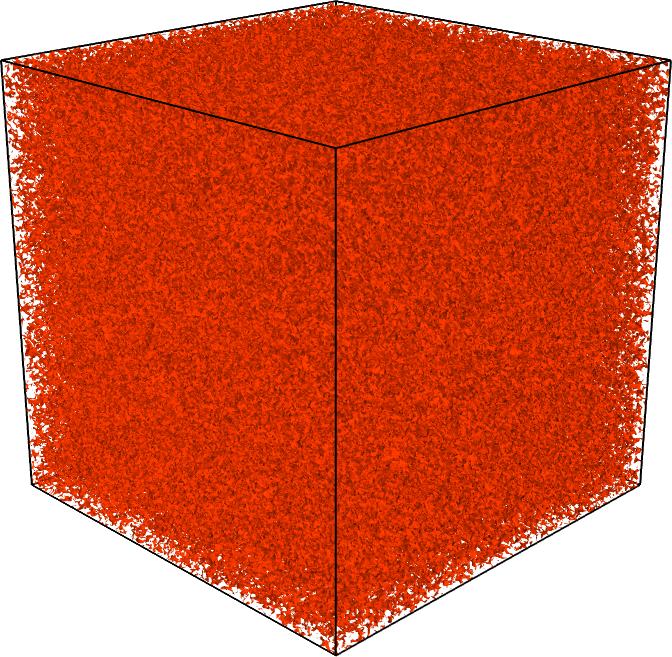
\includegraphics[width=0.4\linewidth]{numerics/figures/mess3d}%
    \begin{minipage}[b]{0.2\linewidth}
      \centering
      \raisebox{3cm}{$\longrightarrow$}
    \end{minipage}% 
    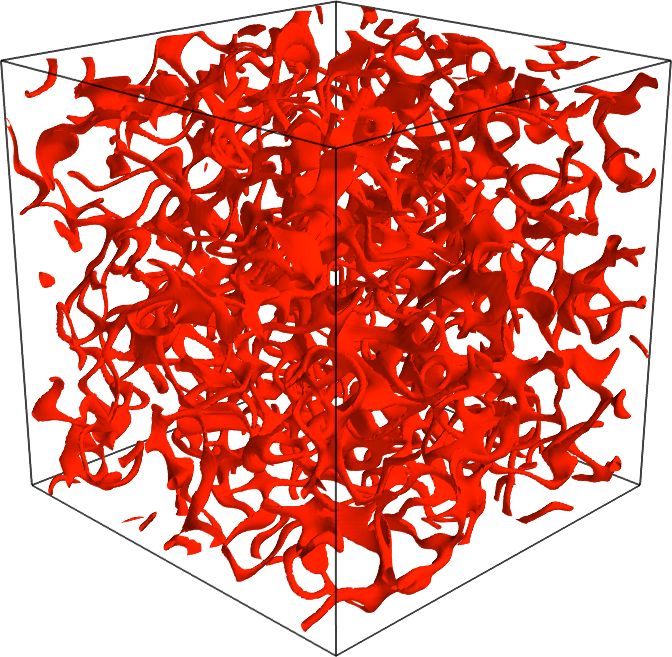
\includegraphics[width=0.4\linewidth]{numerics/figures/clean3d}
  \caption{(Left) Unfiltered wavefunction density, $|\psi|^2$, from a classical-field simulation with condensate fraction $\rho_0/\rho=0.22$ during equilibration. A vortex tangle is present but not visible by direct density visualisation. (Right) Filtered wavefunction density, $|\hat{\psi}|^2$, clearly showing the vortical structures in the gas.}\label{fig:quasicondensatefilter}
  \end{figure}
  	
\section{\label{section:linelength} Evaluation of vortex line-length}
For a given wavefunction, $\Psi$, featuring a vortex distribution, the vortex volume $V_t$ (the total volume associated with the vortex cores) is evaluated by numerical integration of the inside of the vortex isosurface tubes obtained from the filtered density $|\hat \Psi|^2$, with an integration region of the whole numerical box.  Note that the isosurface level should be low enough to pick out vortex cores only (and not, e.g. fluctuations and waves), while large enough to contain sufficient grid points to allow a reasonable numerical evaluation of volume. In this work we use the isosurface level $0.04\langle |\hat{\Psi}|^2 \rangle$ (chosen so as to produce filtered vortex cores that are similar in radius to the true vortex core).  The volume calculation can be written $V_t = \int \Theta(0.04\langle |\hat{\Psi}|^2 \rangle - |\hat{\Psi}({\bf r})|^2)~{\rm d}V$, where $\Theta$ is the Heaviside step function. In practice the calculation of the vortex core volume can be efficiently performed by assigning a value of unity/zero to grid points located within/outside the isosurface tubes and directly integrating the result using the trapezium or Simpson's rule.

The total line length is then deduced by dividing $V_t$ by the cross-sectional area of a vortex core, $A_t$ (in effect, the average cross-sectional area of the isosurface tubes). The measured values of $V_t$ and $A_t$ will depend on the chosen isosurface level but, providing the vortex tubes are well-separated, their ratio (and hence the evaluated line length) will remain constant.  For closely-positioned vortex tubes, the isosurface level can affect whether the tubes appear as two separate tubes, or start to merge, and so will lead to deviations in this ratio.  We have tested the effect of an alternative isosurface value.  For twice the original isosurface value, the difference in the calculated line length is negligible for systems with low vortex density.  For cases with the highest density of vortices, the difference remains less than $10\%$.

\end{chapter}
